\documentclass[a4paper,11pt]{article}

\usepackage[utf8x]{inputenc}
\SetUnicodeOption{mathletters}
\SetUnicodeOption{autogenerated}

\usepackage[italian]{babel}
\usepackage{booktabs}
\usepackage{mathpazo}
\usepackage{graphicx}
\usepackage[left=2cm, right=2cm, bottom=3cm]{geometry}
\frenchspacing

\begin{document}
\noindent {\Large Olimpiadi italiane di informatica 2012 - OII 2012}
\vspace{0.5cm}

\noindent {\Huge La battaglia del convoglio (\texttt{convoglio})}


\section*{Descrizione del problema}
  
\textbf{Nota storica:} tra il 7 e il 10 marzo del 1943 c'è stata
nell'Atlantico  quella che è stata definita \emph{la più grande
battaglia di convogli mai combattuta} . Sottomarini tedeschi si
comunicavano, in maniera cifrata, le posizioni dei convogli americani da
attaccare. Gli alleati conoscevano, ovviamente, le posizioni dei loro
convogli, ed intercettavano le comunicazioni dei tedeschi. Le
informazioni acquisite da queste comunicazioni cifrate, insieme alle
posizioni note dei convogli americani, sono state fondamentali per il
lavoro di Alan Turing a Bletchley Park: qui Turing ha ideato la macchina
Bomba, che ha consentito agli alleati di rompere il codice di Enigma, la
macchina per comunicazioni cifrate dei tedeschi. 
    
Torniamo alla battaglia: un convoglio americano, composto da N navi, è
in viaggio nell'Atlantico. Sottomarini tedeschi si comunicano le
posizioni delle navi e si coordinano per l'attacco. Gli alleati
intercettano le comunicazioni tedesche ma riescono a decrittare solo
parzialmente i messaggi: non sempre si riesce a identificare di quale
nave stiano parlando i tedeschi, e spesso più di una nave americana
potrebbe essere quella a cui fanno riferimento. In particolare, se
indichiamo con $M_{0}$..$M_{N-1}$ gli $N$ messaggi intercettati, e con
$S_{0}$ .. $S_{N-1}$ le $N$ navi della flotta, alla luce di quanto
decodificato ogni messaggio può riferirsi a una o più navi, come si vede
nella figura (dove $N=3$), dove, per esempio, il primo messaggio può
riferirsi sia alla prima ($S0$) che alla terza ($S2$) nave. 
    
\begin{figure}[h!]
  \centering
  \caption{}
  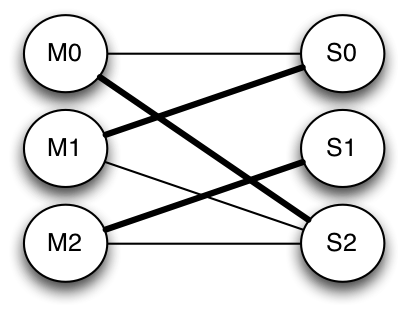
\includegraphics{figura.png}
\end{figure}

    
Turing riesce a trovare una \textbf{corrispondenza univoca} tra i
messaggi e le navi: una corrispondenza in cui \emph{ad ogni messaggio
distinto corrisponde una nave distinta}. Per esempio, le 3 linee a
tratto spesso in figura evidenziano 3 coppie messaggio-nave ($M0-S2$,
$M1-S0$, e $M2-S1$).  Questa è una corrispondenza univoca in quanto:

\begin{itemize}
  \item per ogni $i=1,2,3$ esiste uno ed un solo $j$ tale che la coppia $Mi-Sj$ e' stata inclusa;
  \item per ogni $j=1,2,3$ esiste uno ed un solo $i$ tale che la coppia $Mi-Sj$ e' stata inclusa.
\end{itemize}

Per poter proteggere la flotta bisogna essere sicuri della
corrispondenza, e quindi dobbiamo ora accertarci che non esistano altre
corrispondenze univoche interamente costituite da coppie messaggio-nave
consentite dall'istanza (gli archi in figura, sia in grassetto che in
tratto semplice).  Per esempio, nel caso della Figura 1 esiste anche una
seconda corrispondenza univoca: $M0-S0$, $M1-S2$, $M2-S1$. 
    
Aiutate Turing a capire se la corrispondenza univoca da lui trovata è
anche unica!

\section*{Dati di input}
  
La struttura del file di input è la seguente: la prima riga contiene $2$
interi, $N$ e $M$, che rappresentano, rispettivamente, il numero di navi
(che coincide con il numero dei messaggi intercettati) e il numero
complessivo di possibili corrispondenze tra messaggi e navi. I messaggi
sono identificati da interi compresi tra $0$ e $N-1$, e anche le navi
sono identificate da interi compresi tra $0$ e $N-1$.

Le successive $M$ righe contengono una coppia ordinata di interi
rappresentanti, rispettivamente, un messaggio e una nave corrispondente.
Di queste $M$ righe, le prime $N$ contengono tutti i messaggi e tutte le
navi, e identificano la corrispondenza univoca trovata da Turing.  
    
Con riferimento alla figura, rappresentando i messaggi M0, M1 e M2 con
gli interi 0,1 e 2, e  le navi S0, S1 e S2 con gli interi 0,1 e 2,
l'istanza nella figura viene rappresentata dal file di input a fondo
pagina.

\section*{Dati di output}
  
Se non esiste nessuna altra corrispondenza possibile, il file di output
deve essere costituito da una sola linea, contenente l'intero $-1$.
Altrimenti, se esiste un'altra soluzione, il file di testo contiene $N$
linee, corrispondenti alla soluzione trovata, rappresentata come lista
di coppie di interi, messaggio e nave, ordinate per numero di messaggio.

Con riferimento alla figura, rappresentando i messaggi M0, M1 e M2 con
gli interi 0,1 e 2, e  le navi S0, S1 e S2 con gli interi 0,1 e 2, la
seconda possibile soluzione univoca viene rappresentata dal file di
output a fondo pagina.
 
\section*{Assunzioni}

\begin{itemize}
  \item $N ≤ 100\,000$
  \item $M ≤ 200\,000$
\end{itemize}

\section*{Valutazione delle soluzioni}

\begin{itemize}
  \item  (SubTask 1 - 5 punti) Questo subtask è costituito da una sola istanza: il caso di esempio mostrato qui sotto.
  \item  (SubTask 2 - 16 punti) Nelle istanze di questo subtask si ha che $M=N+2$.
  \item  (SubTask 3 - 22 punti) Nelle istanze di questo subtask si ha che ciascuna nave e ciascun messaggio appare al più $2$ volte nella lista delle possibili corrispondenze (quindi, $M ≤ 2N$).
  \item (SubTask 4 - 27 punti) Nelle istanze di questo subtask $N ≤  3.000$, $M ≤  5.000$ 
  \item (SubTask 5 - 30 punti) Nelle istanze di questo subtask non ci sono vincoli particolari.
\end{itemize}

\section*{Esempi di input/output}
    \noindent
    \begin{tabular}{p{11cm}|p{5cm}}
    \toprule
    \textbf{File \texttt{input.txt}}
    & \textbf{File \texttt{output.txt}}
    \\
    \midrule
    \scriptsize
    \begin{verbatim}
3 6
0 2
1 0
2 1
0 0
1 2
2 2
      \end{verbatim}
    &
    \scriptsize
    \begin{verbatim}
0 0
1 2
2 1
      \end{verbatim}
    \\
    \bottomrule
    \end{tabular}

\end{document}
